%In order to be able to represent objects and their interactions in the global category of higher-order interacting biological entities in terms of diagrams modeled in the local category of such we make use of a generalized form of topology that can be applied to any category meeting a few constraints and that can be specialized to, for example, the case in which objects and morphisms of the category take on a particular type of algebraic structure. The purpose of this construction is to develop a method of defining a {\it covering system} composed of interacting entities in the category representing local interactions that can be used to establish a decomposition of objects in the category representing global interactions that may each rely on a certain type of composition of local interactions with respect to any biological system. We first give a conceptual overview of the standard concepts of {\it sieve}, {\it Grothendieck topology}, {\it site}, and {\it sheaf} for an arbitrary category $\cC$ and then explain how covering sieves on $\mathcal{L}_0$ defined in terms of epimorphic families of morphisms in $\mathcal{L}_1$ provides a Grothendieck topology on $\mathcal{L}_0$, which induces a site and sheaves on $\mathcal{L}_0$, which can be shown to precisely encode the category $\mathcal{L}_1$. The theoretical constraints necessary to ensure the equivalence between information represented in terms of sheaves on the category $\mathcal{L}_0$ and information represented in terms of the category $\mathcal{L}_1$ provide a framework for understanding hierarchically organized systems. The process of transforming the category $\mathcal{L}_0$ into its category of sheaves may then provide broad but precise insight into transitions in hierarchical organization, which is a common property providing a unifying perspective on some of the major transitions in biological evolution.
%
\subsection{sieves}
\begin{frame}
\iftoggle{thmsty}{
\begin{definition}
\label{definition-sieve}
}{}
For any category $\cC$ and $c \in \Ob(\cC)$ a {\it sieve} $S$ on $c$ is a collection in $\Mor(\cC)$ with codomain $c$ such that for $f,g \in \Mor(\cC)$
$$
f \in S \Rightarrow f \circ g \in S
$$
whenever there is a $g \in \Mor(\cC)$ such that $cod(g)=dom(f)$. Any sieve can be restricted to a sieve on the domain of a map whose codomain is the object of the sieve. If $S$ is a sieve on $c$ and $h:d \rightarrow c \in \Mor(\cC)$ with $cod(h)=c$ then
$$
h^* (S) \equiv \{ g \, | \, cod(g)=d, h \circ g \in S \}
$$
is a sieve on $d$.
\iftoggle{thmsty}{
\end{definition}
}
\end{frame}

\begin{frame}
\begin{figure}
\noindent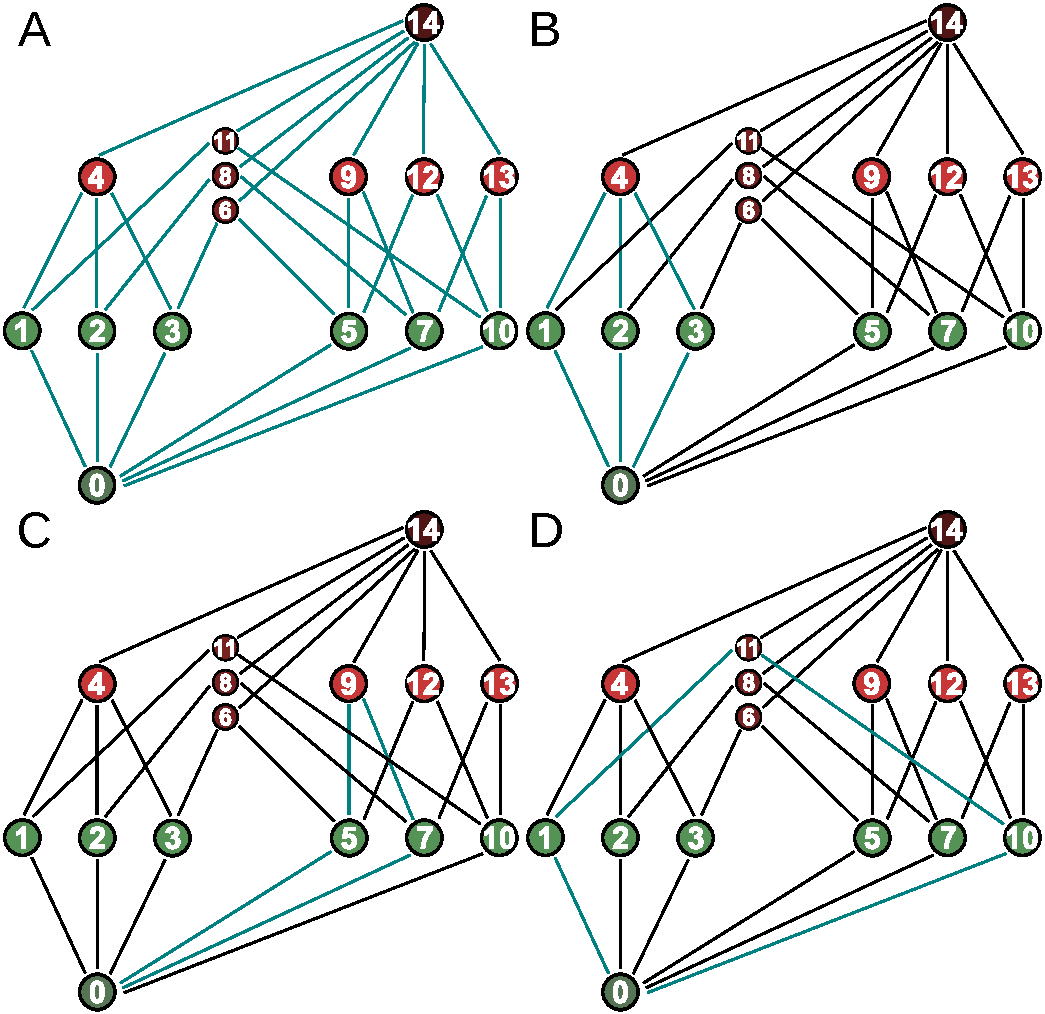
\includegraphics[width=0.4\framewidth]{fig/sieveHasseSetPartitions4.pdf}
\caption{Sieves conceptualized on {\it Hasse diagrams} of an algebraic lattice. All edges are directed from bottom to top. Blue edges are part of a sieve on an object represented by a node in the lattice. Black edges are part of the lattice but not part of the sieve under consideration. (A) shows the maximal sieve on the lattice, which is equivalent to a sieve on object 14. (B) shows a sieve on object 4, (C) shows a sieve on object 9 and (D) shows a sieve on object 11.}
\label{fig:sieve}
\end{figure}
\end{frame}

\begin{frame}
\begin{enumerate}
\item A (maximal) sieve is thus a collection of (all) morphisms impinging on a given object upon which it is defined. 
%Examples of sieves on an algebraic lattice are shown in figure \ref{fig:sieve}. 
\pause \item There is a simple connection between sieves and the Yoneda embedding $PSh:\cC \rightarrow \textit{Sets}^{\cC^{opp}}$. A sieve on $c$ is a subfunctor $Sc \subseteq hom(-,c)$ of the functor in the presheaf category on $\cC$ that is represented by $c \in \Ob(\cC)$. 
\pause \item Placing constraints on such sieves enables the definition of an abstract notion of topology on a category.
\end{enumerate}
\end{frame}

\subsection{Grothendieck topologies}
\begin{frame}
\iftoggle{thmsty}{
\begin{definition}
\label{definition-grothendieck-topology}
}{}
A {\it Grothendieck topology} on a category $\cC$ is a function $J$ that assigns a collection $J(c)$ of sieves on $c$ to each $c \in \Ob(\cC)$ such that conditions of maximality, stability and transitivity are satisfied respectively
\begin{enumerate}
\item the maximal sieve $M_c = \{f \, | \, cod(f) = c\} \in J(c)$,
\item for $S \in J(c)$, $f^*(S) \in J(d)$ for any $f:d \rightarrow c \in \Mor(\cC)$,
\item for $S \in J(c)$, $R \in J(c)$ for any sieve $R$ on $c$ with $f^* (R) \in J(d)$ for all $f:d \rightarrow c \in S$.
\end{enumerate}
Sieves $S$ in $J(c)$ for an object $c \in \Ob(\cC)$ are referred to as $J-covering$ sieves.
\iftoggle{thmsty}{
\end{definition}
}
\end{frame}

\begin{frame}
\iftoggle{thmsty}{
\begin{definition}
\label{definition-basis}
}{}
A {\it basis} for a topology on a category $\cC$ that has pullbacks is a function $B$ that assigns to each object $c \in \Ob(\cC)$ a collection of families $\{c_i \rightarrow c \}$ of morphisms referred to as {\it covering families} in $B(c)$ such that
\begin{enumerate}
\item every family consisting of a single isomorphism $\{ d \cong c \}$ is a covering family in $B(c)$
\item if $\{f_i:c_i \rightarrow c \}$ is a covering family and $g:d \rightarrow c$ is any morphism in $\Mor(\cC)$ then $\{g^* c_i \rightarrow d \}$ is a covering family in $B(d)$ of $d$, which means that the collection of covering families is stable under pullbacks
\item if $\{f_i : c_i \rightarrow c \}_{i \in I}$ is a covering family and $\{ g_{i,j} : c_{i,j} \rightarrow c_i \}_{j \in J_i}$ then the family of composites $\{ f_i \circ g_{i,j} : c_{i,j} \rightarrow c_i \rightarrow c \}_{i \in I, j \in J_i}$ is a covering family in $B(c)$
\end{enumerate}
\iftoggle{thmsty}{
\end{definition}
}
\end{frame}

\begin{frame}
\iftoggle{thmsty}{
\begin{definition}
\label{definition-site}
}{}
A pair $(\cC,J)$ or $(\cC,B)$ consisting of a category $\cC$ and a Grothendieck topology $J$ on $\cC$ or a basis $B$ for such a topology is referred to as a {\it site}. If $S \in J(c)$, then $S$ is a {\it covering sieve} of $c$. If $B$ is a basis on $\cC$, then $B$ is said to {\it generate} a topology $J$ according to the equivalence between the statements that a sieve $S$ is a $J$-cover and that a sieve $S$ contains an associated $B$-cover
$$
S \in J(c) \Longleftrightarrow \exists Q \in B(c), \,\,\, Q \subseteq S.
$$
\iftoggle{thmsty}{
\end{definition}
}
\end{frame}

\subsection{sheaves}
\begin{frame}
\iftoggle{thmsty}{
\begin{definition}
\label{definition-sheaves}
}{}
Given a basis for, $B$, or an explicit Grothendieck topology, $J$, on a category $\cC$ we can define necessary conditions in order for presheaves $P$ in the presheaf category $\textit{Sets}^{\cC^{opp}}$ to be sheaves on the site $(\cC,J)$. If in addition to $P$ we have the sieve $S$ that is a cover of an object $c \in \Ob(\cC)$, then we can define a {\it matching family} for $S$ from elements of $P$ as a function assigning to each $f:d \rightarrow c \in S$ an element $x_f \in P(d)$ such that
$$
\forall g:e \rightarrow d \in \Mor(\cC), \,\,\, x_f \cdot g = x_{fg},
$$
where $x_f \cdot g \equiv P(g)(x_f)$ and $fg \in S$. 
\end{frame}

\begin{frame}
We can further define an {\it almagamation} of a matching family as a single element $x \in P(c)$ such that
$$
\forall f \in S, \,\,\, x \cdot f = x_f,
$$
implying that $P(f)(x)=x_f$ and thus $P(g)(P(f)(x))=x_{fg}$. $P$ is then a {\it sheaf} for $J$ when every matching family for all covers of all objects in $\Ob(\cC)$ have a unique amalgamation. 
\end{frame}

\begin{frame}
A sieve $S$ on an object $c$ is a subfunctor of the functor represented by $c$ under the Yoneda embedding. This is to say that $S \subseteq h^c = hom(-,c)$. In this case, $P$ is a sheaf if and only if for every covering sieve $S$ on $c$ the inclusion $S \hookrightarrow P$ induces an isomorphism $hom(S,P) \cong hom(h^c,P)$. This can also be expressed as the equalizer
\begin{displaymath}
\xymatrix{
P(c) \ar[r]
&
\prod\limits_{f \in S}
P(dom \, f)
\ar@<1ex>[r]^-{p} \ar@<-1ex>[r]_-{a}
&
\prod\limits_{\substack{f,g \,\,\, f \in S \\ dom \, f=cod \, g}}
P(dom \, g)
}
\end{displaymath}
\end{frame}

\begin{frame}
\begin{displaymath}
\xymatrix{
P(c) \ar[r]
&
\prod\limits_{f \in S}
P(dom \, f)
\ar@<1ex>[r]^-{p} \ar@<-1ex>[r]_-{a}
&
\prod\limits_{\substack{f,g \,\,\, f \in S \\ dom \, f=cod \, g}}
P(dom \, g)
}
\end{displaymath}
\noindent for each $c \in \Ob(\cC)$ and each cover $S \in J(c)$. $e$ refers to $e(x)=\{x \cdot f\}_f = \{P(f)(x)\}_f$, $p$ refers to $p( \mathbf{x} )_{f,g} = x_{fg}$, and $a$ refers to $a( \mathbf{x} )_{f,g} = x_f \cdot g$ for $\mathbf{x} = \{ x_f \}_{f \in S}$. Given that the equalizer condition, $p \circ e = a \circ e \Leftrightarrow p=a$, is satisfied for a cover $S$ then $P$ is a sheaf with respect to the cover $S$.
\end{frame}

\begin{frame}
Finally, to express the sheaf condition in terms of a basis $B$ for a topology $J$ generated by $B$ on a category $\cC$ having pullbacks. If $Q = \{ f_i : c_i \rightarrow c \}_{i \in I}$ is a B-cover of $c$ a family of elements $x_i \in P(c_i)(i \in I)$ is a matching family for $Q$ if $ x_i \cdot \pi_{ij}^1 = x_j \cdot \pi_{ij}^2$ for all $i,j \in I$. $\pi^1$ and $\pi^2$ are defined as
\begin{displaymath}
\xymatrix{
c_i \times_c c_j \ar[r]^-{\pi_{ij}^2} \ar[d]_{\pi_{ij}^1} & c_j \ar[d]^{f_j} \\
c_i \ar[r]^{f_i} & c
}
\end{displaymath}
\end{frame}

\begin{frame}
\noindent Now again, a presheaf $P \in \textit{Sets}^{\cC^{opp}}$ is a sheaf for the topology $J$ generated by the basis $B$ if and only if for any cover $\{ f_i : c_i \rightarrow c \}_{i \in I}$ in $B$ any matching family $\{ x_i \}_i$ has a unique amalgamation $x \in P(c)$ such that $x \cdot f_i = x_i$ for all $i \in I$. This condition can also be expressed in terms of a diagram that is an equalizer
\begin{displaymath}
\xymatrix{
P(c) \ar[r]
&
\prod\limits_{i \in I}
P(c_i)
\ar@<1ex>[r]^-{p_1} \ar@<-1ex>[r]_-{p_2}
&
P(c_i \times_c c_j)
}
\end{displaymath}
\noindent The morphism $e$ refers to $e(x) = \{ x \cdot f_i \}_i$, $p_1$ refers to $p_1(\{ x_i \})_{i,j} = x_i \cdot \pi_{ij}^1$, and $p_2$ refers to $p_2(\{x_i\})_{i,j} = x_j \cdot \pi_{ij}^{2}$.
\iftoggle{thmsty}{
\end{definition}
}
\end{frame}

\begin{frame}
We are now able to explain how covering sieves on $\mathcal{L}_0$ defined in terms of epimorphic families of morphisms in $\mathcal{L}_1$ provides a Grothendieck topology on $\mathcal{L}_0$, which induces a site and sheaves on $\mathcal{L}_0$, which can be shown to precisely encode the category $\mathcal{L}_1$.
\end{frame}